\let\oldvec\vec % Store \vec in \oldvec
\documentclass{llncs}
\let\vec\oldvec % Restore \vec from \oldvec

\usepackage[utf8]{inputenc}
\usepackage{url}
\usepackage{cite}
\usepackage{hyperref}
\usepackage{graphicx}
\usepackage{acronym}
\usepackage{float}
\usepackage{pgfgantt}
\usepackage{fixltx2e}
\usepackage{mathtools}
\usepackage{amsmath}
\usepackage{booktabs}
\usepackage{array}
\usepackage{subcaption}
\usepackage{geometry}
\usepackage{pdflscape}
\usepackage{placeins}

%% REDUCE TEXT SIZE
% \addtolength{\textwidth}{1cm}
% \addtolength{\textheight}{1cm}

%% change bullet style
\renewcommand{\labelitemi}{$\bullet$}

\begin{document}

% HappiTweets
\title{Happiness in the U.S.: Measuring the Sentiment of Geolocated Tweets}

\author{João Ferreira Loff \newline \email{joao.loff@tecnico.ulisboa.pt}}
\institute{Universidade de Lisboa - Instituto Superior Técnico}
\date{June 2, 2014}

\maketitle

\begin{abstract}
Individual happiness is a fundamental societal metric. Normally measured through self-report or survey-like schemes, happiness has often been indirectly characterized and overshadowed by more readily quantifiable economic indicators. In this paper I analyze data from the micro-blogging site Twitter and generate a happiness map and ranking for all Continental U.S. states and counties. I do so by combining (1) a massive, geotagged data set comprising over 233 million tweets in 2012 and (2) comparing those results with the annually happiness index made by Gallup-Healthway. In measuring happiness I use the aproched introduced by Dodds and Danforth in 2009 \cite{Dodds2009}, and greatly expanded upon by \cite{Dodds2011,Mitchell2013}. I found out that there is a good enough correlation between my approach and Gallup-Healthway survey. Most important (and never hear of) conclusion I reached was that there is a very strong correlation between the number of tweets from a state and its happiness ranking, unveiling that Twitter usage is a very strong variable to take into account regarding state happiness.
\end{abstract}


\section{Introduction}

Numerous studies on well-being are published every year. The UN’s 2012 World Happiness Report attempts to quantify happiness on a global scale using a `Gross National Happiness' index which uses data on rural-urban residence and other factors \cite{Layard2013}. In the U.S., Gallup and Healthways produce a yearly report on the well-being of different states, cities, communities and congressional districts, with a well-being index based on continual polling and survey data \cite{GallupHealthway2013}. Another known initiative is the Happy Planet Index, introduced by the New Economics Foundation and that measures human well-being and environmental impact \cite{TheNewEconomicsFoundation2012}.

While these and other approaches to quantifying the sentiment of a population (be either a state or a city) as a whole rely almost exclusively on survey data, there are now a range of complementary, remote-sensing methods available to researchers. For the social sciences, the explosion in the amount and availability of data relating to social network use in the past 10 years has led to a collective, open recording of an enormous number of transactions, interactions, and expressions, marking a clear transition in our ability to quantitatively characterize, and thereby potentially understand, previously hidden as well as novel micro-scale mechanisms underlying socio-technical systems \cite{Miller2011}. This has driven a rapid increase in the application of data-driven techniques to the social sciences and sentiment analysis of large-scale populations.

My overall aim in this paper is to investigate how geographic place correlates with societal levels of happiness. In particular, I will be examining happiness dynamics at the level of U.S. states and counties, asking if it is possible to accurately measure the overall average happiness of people located in states and counties. My methodology for answering the first question uses word frequency distributions collected from a large corpus of messages posted on Twitter, with individual words scored for their happiness independently by users of Amazon’s Mechanical Turk service. This technique was introduced by Dodds and Danforth in 2009 \cite{Dodds2009}, and greatly expanded upon in \cite{Dodds2011}, as well as used and tweaked by others such as \cite{Mitchell2013}.

Among many results, I generated three choropleths: (1) one with the distribution of happiness score by U.S. state, (2) another that uses the same technique that Gallup-Healthway uses fo their reports, and I use this choropleth to compare my results with their index (3) and finally one with the same set of happiness score, but distributed by U.S. counties. In fact, many of the other results have a focus on the comparison between my results and Gallup-Healthway report. Finally, a striking correlation value appeared between the number of tweets and the position in the happiness state ranking, the more tweets a state has the more sad it appears to be.

My paper is structured as follows. In Section \ref{sec:rw} I describe the previous related work related to my sutdy. In Section \ref{sec:datasets}, I describe the data sets I used. In Section \ref{sec:meth} I describe my methodology for measuring happiness. In Section \ref{sec:results} I measure the happiness of different states and counties and determine the happiest and saddest states in the U.S., and at the same time I compare my results with the Gallup-Healthways Well-being Index \cite{GallupHealthway2013}. I conclude with a discussion and a reference for future work in Section \ref{sec:conc}.

\section{Related Work}
\label{sec:rw}

In \cite{Mitchell2013,Dodds2011,Frank2013,Bliss2012} the overall aim is to investigate how geographic place correlates with and potentially influences societal levels of happiness. In particular they ask if it is possible to (a) measure the overall average happiness of people located in U.S. states and cities, and (b) explain the variation in happiness across different states and cities. The first question is answered using word frequency distributions collected from a large corpus of \emph{tweets} posted on Twitter, with individual words scored for their happiness using the technique by Dodds et al. \cite{Dodds2009}, which is an improvement of the original ANEW approach \cite{Bradley1999}. To answer the second question of happiness variability, they examine how individual word usage correlates with happiness and various social and economic factors, using the `word shift graph' technique developed in \cite{Dodds2011,Dodds2009}, and socioeconomic census data to attempt to explain the usage of certain words. To obtain a score for a given tweet T containing N unique words, they calculate the average happiness $h_{avg}$ using an weighted average of the number of times a word occurs in T, multiplied by the the $h_{avg}$ of that specific word. They then divide the weighted average of all the words, with the total number of detected LabMT words. Finally they used the average of the scores, to achieve the happiness scoring of a given state. Some of the most important results from these studies are:
\begin{itemize}
\item From \cite{Mitchell2013}, social media may potentially be used to estimate real-time levels and changes in population-level measures such as obesity rates;
\item From \cite{Bliss2012}, more well connected users write happier status updates;
\item From \cite{Frank2013}, expressed happiness increases logarithmically with distance from an individual’s average location;
\item From \cite{Dodds2011}, it was proved that the seven day week cycle is an historical and cultural artifact.
\end{itemize}

In \cite{Bertrand2013} they use Twitter to study the fine-grained geography and dynamics of sentiment in the greater New York City area, identifying areas and times of positive and negative sentiment. They develop a classifier based upon supervised learning specifically tuned for 140-character Twitter messages, using key words, phrases and emoticons to determine the mood of each tweet. They use labeled tweets regarding the presence of emoticons, to build two classifiers: one to classify whether or not a tweet is positive, and another to classify whether or not a tweet is negative. This method, combined with geotagging provided by users, enabled them to gauge public sentiment on extremely fine-grained spatial and temporal scales. They find that public mood is generally highest in public parks and lowest at transportation hubs, and locate other areas of strong sentiment such as cemeteries, medical centers, a jail, and a sewage facility. Sentiment progressively improves with proximity to Times Square. Periodic patterns of sentiment fluctuate on both a daily and a weekly scale: more positive tweets are posted on weekends than on weekdays, with a daily peak in sentiment around midnight and a nadir between 9:00 a.m. and noon.

In \cite{Connor2010} they connect measures of public opinion derived from polls with sentiment measured from analysis of text from Twitter. They explicitly link measurement of textual sentiment in microblog messages through time, comparing to contemporaneous polling data. In this preliminary work, summary statistics derived from extremely simple text analysis techniques are demonstrated to correlate with polling data on consumer confidence and political opinion, and can also predict future movements in the polls. They derive day-to-day sentiment scores by counting positive and negative messages. Positive and negative words are defined by the subjectivity lexicon from OpinionFinder. They do not use the lexicon's distinctions between weak and strong words. They define the sentiment score on day as the ratio of positive versus negative messages on the topic, counting from that day's messages.

In \cite{Schwartz2013} they address subjective well-being, as measured by life satisfaction. They correlated the words within Twitter messages (in the form of LDA-generated word topics) mapped to U.S. counties, with the results for life satisfaction, as measured by questionnaires answered in those counties. Their goal is not to count positive sentiment words, like the studies above, but to study the language of well-being, to better understand the multiple components that contribute to it, i.e. they find the lexica and topics that correlate with life satisfaction as measured in questionnaires. They also add several control variables such as age, sex, minority, income, education. Finally, they run all the variable - the lexica, the topics and the control variables - through a LASSO linear regression with life satisfaction over counties. The surprising fundamental result of this paper is that they can predict (on average) the happiness of one set of people (those who answered the LS questionnaires) from the tweets of other people (people in the same county).

\section{Datasets}
\label{sec:datasets}

I examine a corpus of over 232 million tweets gathered from all over the world during the calendar year of 2012. After an initial parsing effort, I reduced the data set to have only geotagged tweets, which is near 0.78\% of the whole data set (less than 1.8 million tweets). For the present study, I focus only on the geotagged tweets located in the Continental U.S., excluding Alaska and Hawaii, which is near 27\% of the geotagged tweets (less than 0.5 million tweets).

Polygonal areas corresponding to the different U.S. were obtained from the state data set that is available from the \emph{maps} package for the R system for statistical computing \footnote{available at http://cran.r-project.org/web/packages/maps/}.

To measure sentiment (hereafter happiness) in these areas from the corpus of words collected, I use the Language Assessment by Mechanical Turk (LabMT) word list (available online in the supplementary material of \cite{Dodds2011}), assembled by combining the 5'000 most frequently occurring words in each of four text sources: Google Books (English), music lyrics, the New York Times and Twitter. A total of  10'233 of these individual words have been scored by users of Amazon’s Mechanical Turk service on a scale of 1 (sad) to 9 (happy), resulting in a measure of average happiness for each given word \cite{Kloumann2012}. For example, `rainbow' is one of the happiest words in the list with a score of $h_{avg}$ = 8.1, while `earthquake' is one of the saddest, with $h_{avg}$ = 1.9. Neutral words like `the' or `thereof' tend to score in the middle of the scale, with $h_{avg}$ = 4.98 and 5 respectively.

Fig. \ref{fig:tweets_by_state} presents (i) the total number of tweets per state, (ii) the number of tweets containing LabMT words, and (iii) the percentage of tweets containing LabMT words. In median $75\%$ of the total tweets have LabMT words.

\begin{figure}
\centering
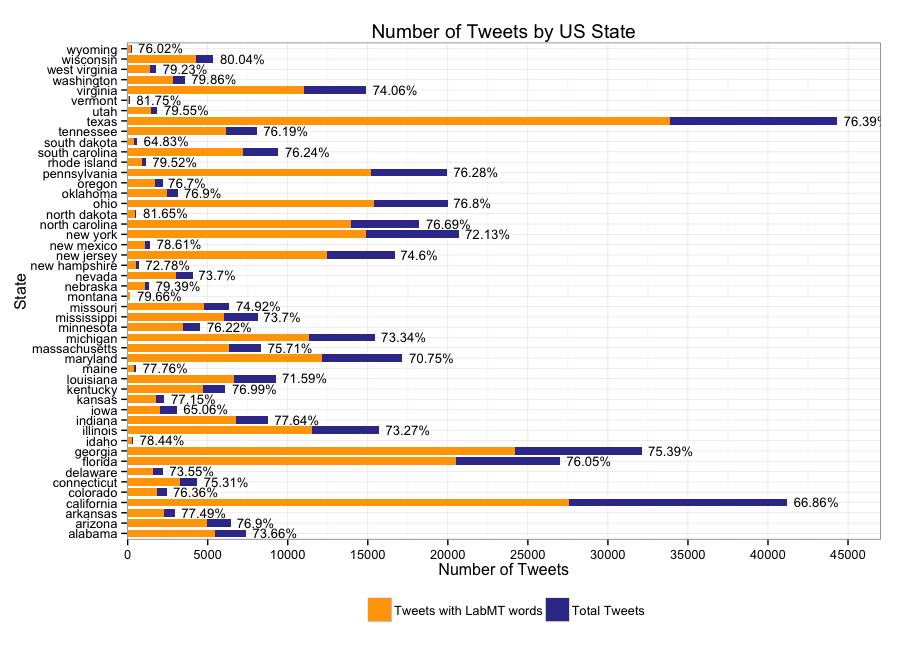
\includegraphics[width=\textwidth]{images/tweets_by_state}
\caption{Stacked bar chart for the number of tweets by U.S. state. In blue the total number of tweets, and in orange the number of tweets with words from the LabMT corpus of words. In front of each bar I have the percentage of tweets that have LabMT words.}
\label{fig:tweets_by_state}
\end{figure}

Finally I will be using the 2012 Gallup-Healthways Well-being Index results \cite{GallupHealthway2013} \footnote{available at http://info.healthways.com/wbi2013}. This study has an \emph{Overall Well-Being Index} that I will use as a happiness index to correlate with our results.

\FloatBarrier
\section{Methodology}
\label{sec:meth}
My section is structured as follows. In Section \ref{sec:meth1} I detail how I processed the tweets with the LabMT approach from \cite{Dodds2011}. In Section \ref{sec:meth2} I present how I processed the placement of each geotagged tweets in its appropriate state. In Section \ref{sec:meth3} I present some processing I made regarding the Gallup-Healthway Well-Being Index. In Section \ref{sec:meth4} I explain how I reached a single score for each state. In Section \ref{sec:meth5} I present some visualization techniques I adopted to present the results from my work.

\subsection{LabMT Tweet Processing}
\label{sec:meth1}
As stated in Section \ref{sec:datasets}, to measure sentiment (hereafter happiness) in the areas from the corpus of words collected, I use the Language Assessment by Mechanical Turk (LabMT) word list \cite{Dodds2011}. This word list has a total of roughly 10'000 of individual words, which have been scored on a scale of 1 (sad) to 9 (happy), resulting in a measure of average happiness for each given word \cite{Kloumann2012}. For a given text T containing N unique words, I calculate the average happiness $h_{avg}$ by:
\begin{align*}
h_{avg}(T) = \frac{\sum_{i=1}^{N} h_{avg}(w_i)f_i}{\sum_{i=1}^{N} f_i} \tag{1}\label{eq:1}
\end{align*}
where $f_i$ is the frequency of the $i$th word $w_i$ in $T$ for which I have a happiness value $h_{avg}(w)$, and $p_i = f_i/\sum_{i=1}^{N}f_i$ is the normalized frequency of word $w_i$. This is a similar approach of the original ANEW research \cite{Bradley1999}, that's explained in \cite{Dodds2009}.
This method makes no attempt to take the context of words or the meaning of a text into account. While this might lead to difficulties in accurately determining the emotional content of small texts, it was proved that for sufficiently large texts this approach nonetheless gives reliable (if eventually improvable) results \cite{Dodds2011,Mitchell2013,Dodds2009,Kloumann2012}.
Following Dodds et al. \cite{Dodds2011}, I remove all words $w_i$ for which the happiness score falls in the range $4 < h_{avg}(w_i) < 6$ when calculating $h_avg(T)$. Removal of these neutral words has been demonstrated to provide a suitable balance between sensitivity and robustness in \cite{Dodds2011}. Following \cite{Mitchell2013}, to avoid the problem that some states have happier names than others I removed (a) each state name from the calculation for $h_{avg}$; and (b) all variants of the racial pejorative or ‘N-word’, since variants of this word have very low happiness values, and consequently were found to be highly influential in determining the state happiness score, however upon examining individual tweets \cite{Mitchell2013} found that this word appeared to be being used in conversation as a more colloquial stand in for the word `friend', and not in fact in any particularly negative sense, therefore the word was unfairly biasing \cite{Mitchell2013} the results towards the negative and removed it.

To increase the amount of tweets considered in the study, I also processed the same data set but using a Spanish list of words resulting from work by \cite{Redondo2007} \footnote{word list available at http://link.springer.com/article/10.3758\%2FBF03193031}. This process allowed me to increase the number of tweets in near 40'000. To avoid tweets with score with both lists, leading to duplicated tweets, I only choose the score from the language were it was detected more words. Example, if I have this tweet: ``You are a very good friend, compadre!'', even if I have the one word from the Spanish list (`compadre'), there are 2 words form the English list (`good', `friend'). Therefore, I choose to score this tweet with the English word list.


\subsection{Geolocating Tweets}
\label{sec:meth2}
Each geotagged tweet from the data set was processed in order to extract its latitude and longitude coordinates, searching for those
fields in the JSON object corresponding to each Twitter message \footnote{available at https://dev.twitter.com/docs/platform-objects/tweets}. After stripping those two fields, and to be able to match each tweet to a U.S. state, I used the \emph{sp} R package \footnote{available at http://cran.r-project.org/web/packages/sp/} more specifically the \emph{over} function, which does consistent spatial overlay for points, grids and polygons, i.e., if a latitude/longitude point $x$ and a polygon $P$ representing a state is given, the over function returns \emph{true} or \emph{false}, if that point is inside the polygon - if a certain tweets belongs to a certain state.


\subsection{Gallup-Healthway Score}
\label{sec:meth3}
I will correlate our happiness results with with the 2012 Gallup-Healthways Well-being Index \cite{GallupHealthway2013} \footnote{available at http://info.healthways.com/wbi2013}. Since LabMT score goes from 1 to 9, I had to rescale the Gallup-Healthways Overall Well-Being Index from a percentage scale (0-100) to the 1-9 point scale used in the LabMT lexicon. For this I used the known `typical' function to rescale values from one range to another:
\begin{align*}
rescale_(x) = \frac{(b-a)(x-min)}{max-min} + a \tag{2}\label{eq:2}
\end{align*}
where, for our case: $min = 0$, $max = 100$, $a = 1$ and $b = 9$.


\subsection{Score by U.S. State}
\label{sec:meth4}
After having all tweet associated with a state, I had to choose one of the three central tendency statistics that allowed me to get a score for a whole state state, using either the \emph{mean}, \emph{median} or the \emph{mode}. To choose between them I plotted the histograms for the score distributions of some states (see Fig. \ref{fig:tweets_distribution}), to observe the patterns for tweet distribution, and I calculated the correlation factor between those three statistics and the Gallup-Healthway Index.

\begin{figure}
\centering
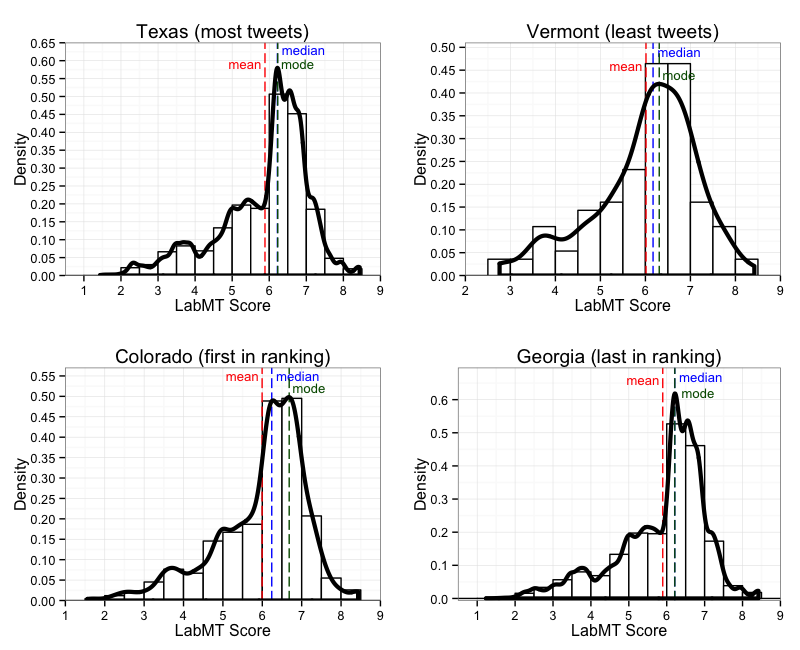
\includegraphics[width=\textwidth]{images/tweets_distribution}
\caption{Histograms and density lines for Texas (state with most tweets), Vermont (state with least tweets), Colorado (first in state happiness ranking) and Georgia (last in happiness state ranking). Vertical red line is the mean of the scores, vertical blue line is the median of the scores, and vertical green line is the mode for the scores.}
\label{fig:tweets_distribution}
\end{figure}

An initial analysis lead me to choose the \emph{mode} because the correlation was the highest. The mode method I used, the most common one, was the Pearson correlation coefficient. The Pearson correlation is a measure of the linear correlation (dependence) between two variables X and Y, giving a value between +1 and -1 inclusive, where 1 is total positive correlation, 0 is no correlation, and -1 is total negative correlation. It is widely used as a measure of the degree of linear dependence between two variables. It is defined as the covariance of the two variables divided by the product of their standard deviations. \cite{Pearson2006}

I limited the mode density function interval to $[1,9]$, the range of values of the LabMT word scores, and used a adjust (smooth) factor of $0.80$. This allowed me to achieve a correlation of approximately $0.45$. Taking in consideration what has been shown in other studies \cite{Dodds2011,Frank2013,Bliss2012}, that a correlation value between studies near similar to this one are usually around the $0.50$ mark, I can conclude that our approach is yielding very good results. The correlation results are shown below:
\begin{flalign*}
    & X = \textrm{Gallup-Healthway Well-Being Index score by state} \tag{3}\label{eq:3}\\
    & cor(X , Y) = 0.187 ,\textrm{ with Y = mean of LabMT tweet scores by state} \\
    & cor(X , W) = 0.029 ,\textrm{ with W = median of LabMT tweet scores by state} \\
    & cor(X , Z) = 0.448 ,\textrm{ with Z = mode of LabMT tweet scores by state}
\end{flalign*}


\subsection{Visualization}
\label{sec:meth5}
Finally I present our results using one of the visualization methods discussed in \cite{Nollenburg2007}, which is also used in \cite{Mitchell2013,Dodds2011}, the Choropleth map.
Th Choropleth map uses the graphic variables describing properties of color or texture to show properties of non-overlapping areas, such as provinces, districts, or other units of territory division. A number of categories is mapped to distinct colors or textures which are used to fill the areas accordingly. For the colors used on our choropleths, I used the \emph{RdYlGn} palette from the \emph{RColorBrewer} R package \footnote{available at http://cran.r-project.org/web/packages/RColorBrewer/}, which has a set of default color palettes based on the work done by \cite{Harrower2003} \footnote{available at http://colorbrewer.org}. I presented our maps using the \emph{globular projection} detailed in \cite{Bolstad2012}.

\FloatBarrier
\section{Results}
\label{sec:results}

First I plot the average happiness of all Continental U.S., excluding Alaska and Hawaii in Fig. \ref{fig:scores_by_state}. In this chart I plot our results redefining the scale so I get a greater amount of different colors near the mean value of our state scores. This way I avoid using an uniform scale, that causes most of the states to be with the same color. Our scale is an approximation of a Normal Distribution, but in a ad-hoc manner: $scale = \langle min, mean - (sd/2), mean - (sd/3) , mean, mean + (sd/3), mean + (sd/2), max \rangle$. The result is a scale that increases the amount of different colors near the mean, and uses the same ones in the extremities.

\begin{figure}
\centering
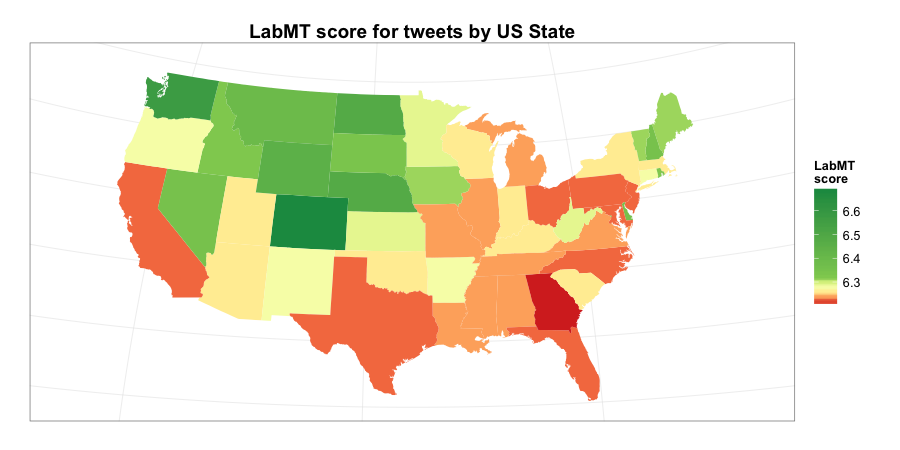
\includegraphics[width=\textwidth]{images/scores_by_state}
\caption{Choropleth showing \emph{mode} word happiness for geotagged tweets in all Continental U.S. states collected during the calendar year 2012. The happiest 5 states, in order, are: Colorado, Washington, Nebraska, North Dakota, Wyoming. The saddest 5 states, in order, are: Georgia, Texas, Pennsylvania, Ohio, North Carolina. The full state ranking is shown in Appendix section.}
\label{fig:scores_by_state}
\end{figure}
\FloatBarrier

At such a coarse resolution there is little variation between states, which lie between $0.09$ and $0.38$. The $h_{avg}$ of the mean value for the entire U.S. is $6.30$ and the standard deviation has a value of $0.09$. The top 5 states are the ones that are far apart from the mean value, are in average 0.23 above the mean. The happiest state is Colorado with a score of $h_{avg} = 6.68$ and the saddest state is Georgia with a score of $h_{avg} = 6.21$. The striking observation that I take from the ranking is the high correlation between the state's position in the ranking and the number of tweets of that state, $cor(\textrm{number of tweets}, \textrm{ranking}) = 0.77$, and also a high correlation between the score and the number of tweets, $cor(\textrm{number of tweets}, \textrm{LabMT score}) = -0.48$. This means that the more tweets a state has the lower it will be in the ranking (and the sadder it will appear to be). In fact, if I split our states into equal parts (6 states each group), I can clearly see the average number of tweets per group increases as I lower in the ranking (see Table \ref{tab:tab1}).

\begin{table}
\centering
\begin{tabular}{>{\centering\arraybackslash}m{1in}  >{\centering\arraybackslash}m{1in}}
\toprule
Ranking    & Average number of tweets \\
\midrule
1-12th     & 1376                     \\
13-24th    & 4391                     \\
25-36th    & 5344                     \\
37-48th    & 14479                    \\
\bottomrule
\end{tabular}
\linebreak
\caption{Average of tweets per position in state ranking}
\label{tab:tab1}
\end{table}
\FloatBarrier

Another interesting way to look at the data is to emulate the style that Gallup-Healthway uses for the choropleth in their report. They split up the scores per state in five quintiles, coloring them in the map. For the sake of easier comparison, I present both the original and our own choroplet using the same scheme Gallup-Healthway uses.

Even tough there is no striking resemblance between the two charts in Fig. \ref{fig:gallup_vs_labmt}, if you take into account the little variation of the scores that I discussed before, I can assume that a state could easily be on another quintile (except the top 5, as I also discussed before). In the Southeast I have similar results, with some of the states that should be in the 4th Quintile are in the 5th. Northeast section is very far apart with many of the values on the 4th/5th Quintile when they should be in the 3rd/2nd, still in the north part there's some improvement. Midwest section has yet again some striking resemblance between the 1st and 2nd Quintile states. Southwest state also have some resemblance with some states switching between the 3rd and 5th Quintile. Finally, the West appears similar with some states switching between the 1st and 2nd Quintile, but with a staggering difference in California. In fact, there are very few states that jump more than 3 Quintiles in their classification.

\begin{figure}
\begin{subfigure}[b]{\textwidth}
\centering
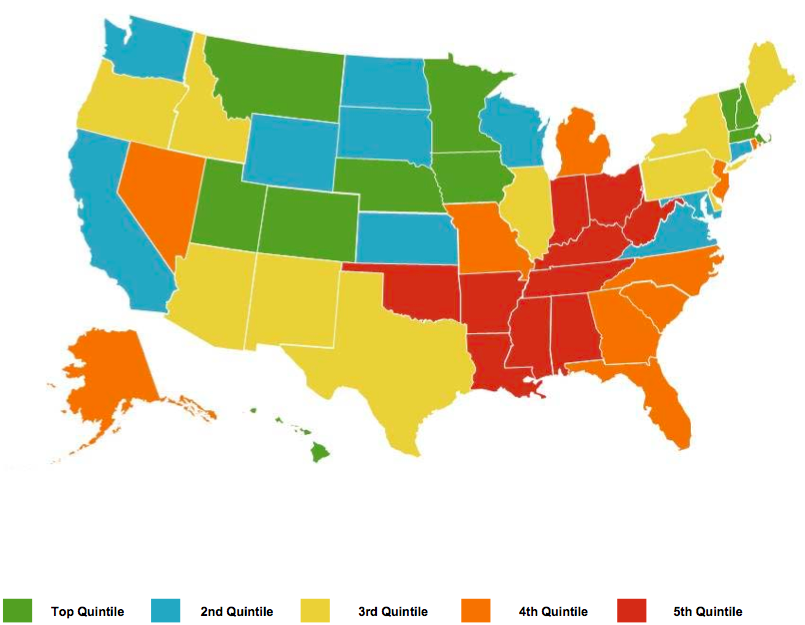
\includegraphics[width=\textwidth]{images/gallup_2012}
\end{subfigure}
\begin{subfigure}[b]{\textwidth}
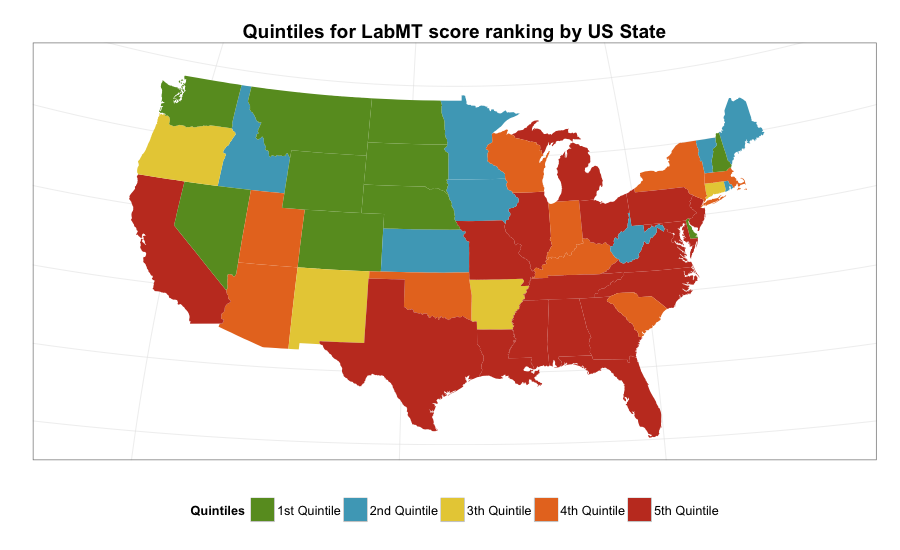
\includegraphics[width=\textwidth]{images/scores_by_state_gallup_style}
\end{subfigure}
\caption{Gallup-Healthway Well-Being Index choropleth vs Our own choropleth using the same quintile schema as well as the same color code.The happiest 5 states for Gallup-Healthway study are, in order, are: Colorado, Minnesota, Utah, Vermont, Nebraska. The saddest 5 states, in order, are: Arizona, Tennessee, Mississippi, Kentucky, West Virginia. The full state ranking is shown in Appendix section. Source \cite{GallupHealthway2013}}
\label{fig:gallup_vs_labmt}
\end{figure}

You can attest that analyzing the ranking differences in the bump chart in Fig. \ref{fig:bump_chart} that compares the changes in ranking between the LabMT approach and Gallup-Healthway score. What I aim with this graph is a high number of straight (or almost straight) lines. Those indicate that the rank stayed the same (or almost the same) in both approaches. As I expected (since I achieved a correlation of approximately $0.45$), a reasonable amount of lines are straight. Regarding the lines that aren't straight, I can observe that they connect extremes of the ranking (with rare exceptions).

Regarding score difference in spite of the little variation there is our scores, the average difference between Gallup-Healthway score and is just 0.02. What happens is that, and I can verify that analyzing Fig. \ref{fig:differences} (in Appendix A), I either have very small differences (in the range of few hundredths) or I have very large differences (in the range of several tenths). This leads to situations I can see in Fig. \ref{fig:bump_chart}, where many times I see a state changing very few positions in ranking and other times changing many positions.

\begin{figure}
\centering
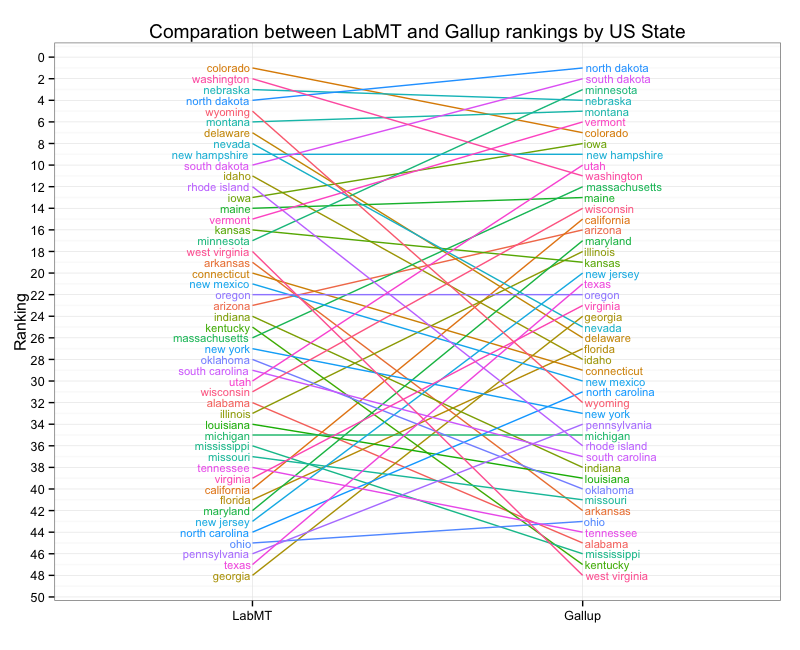
\includegraphics[width=\textwidth]{images/bump_chart}
\caption{Bump chart that compares the changes in ranking between the LabMT approach and Gallup-Healthway score. On the right column you have the ranking from our approach using LabMT word list. On the left column I have the Gallup-Healthway ranking for the calendar year of 2012 \cite{GallupHealthway2013}, minus the states that I didn't considered in our study, i.e., Alaska and Hawaii.}
\label{fig:bump_chart}
\end{figure}

Approaches similar to Gallup-Healthway report, i.e. approaches that quantifying the sentiment of a population that rely almost exclusively on survey data, are limited in the scale they are made. Using this approach it would be very difficult, if not impossible, to use the exact same data set to analyze a different scale, e.g. at the level of counties. Currently Gallup-Healthway focus their research on State, Community and (some) cities. Meanwhile using my approach and dataset, I could be able to reach a level of detail based on street if necessary. I demonstrate this with analysis with a chropleth at the level of U.S. counties (Fig. \ref{fig:scores_by_county}), clearly showing the huge potential of these types of approaches when compares with survey-like approaches.

The scale is the same as in the original choropleth (Fig. \ref{fig:scores_by_state}) so the comparison between the two maps is easier. This forced me to cap the values used in the county map to the minimum and maximum score values that I found in the state map. There is a great amount of dispersion regarding the number of tweets by county, with a mean of 230 tweets per county but with a sd of 675. That's why I observe weird patterns like the state of California, where the counties are mainly green but the red counties are the ones with the most tweets. When I move to a coarser scale, those counties with the highest number of tweets will contribute more towards the mode score, leading to a shift in the overall state score.

\begin{figure}
\centering
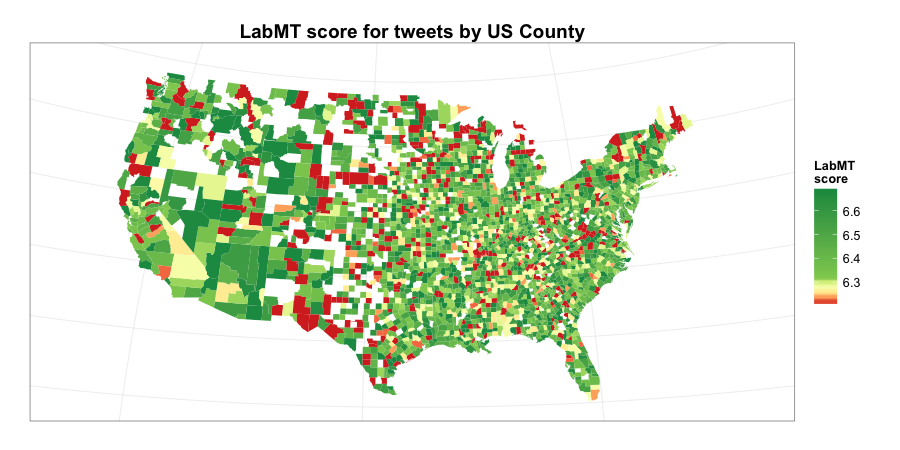
\includegraphics[width=\textwidth]{images/scores_by_county}
\caption{Choropleth showing \emph{mode} word happiness for geotagged tweets in all Continental U.S. counties collected during the calendar year 2012. The scale is the same as the one used in Fig. \ref{fig:scores_by_state}, with values capped to the range of scores of the state.}
\label{fig:scores_by_county}
\end{figure}


\FloatBarrier
\section{Discussion and Future Work}
\label{sec:conc}

In this paper I have examined word use in urban areas in the U.S., using a simple mathematical method which has been shown to have great flexibility, sensitivity and robustness. I have used this tool to map areas of high and low happiness and score individual states (and also counties) for average word happiness.

My state ranking is backed up with a strong correlation between my results and the results of Gallup-Healthways report but also with the results in \cite{Mitchell2013}. In fact, if you consider that the correlation between \cite{Mitchell2013} and the Gallup-Healthway report is $0.50$, my correlation value of $0.48$ for the same report, is an excellent value for the scale of my research in comparison with \cite{Mitchell2013} study. Meanwhile, the correlation between my study and \cite{Mitchell2013} is also of $0.45$. This indicates what have been shown in other studies \cite{Dodds2011}, that a correlation value between studies similar to these are usually around the $0.50$ mark, and if I reach such a value I can consider that our approach is yielding good results and that's robust enough.

The one conclusion that I take from our study, that I didn't find in any of the other related work is the very high correlation between the amount of tweets and the ranking (or score) of a state. The value of $0.77$ value that I found clearly indicates that Twitter usage might be correlated with happiness in that state. A different interpretation I can take form this value, is that the more individuals use Twitter, the more they write messages with negative connotation. And who uses less, uses Twitter to broadcast messages with positive connotation.

There are a number of legitimate concerns to be raised about how well the Twitter data set can be said to represent the happiness of the greater population. Roughly 15\% of online adults regularly use Twitter, and 18-29 year-olds and minorities tend to be more highly represented on Twitter than in the general population \cite{Smith2012}. Furthermore, the fact that the collected sample is small compared with the overall Twitter usages, and that the geotagged tweets are even less means that our data set is a non-uniform subsample of statements made by a non-representative portion of the population. One could improve the amount of geotagged tweets, considering for the non-geotagged tweets that they were made from the city the user filled in its Twitter registration form.

In this work I have only scratched the surface of what is possible using this particular dataset. I have not examined whether or not these methods have any predictive power—future research could look at how observed changes in the Twitter data set, predict changes in the underlying social and economic characteristics measured using traditional survey methods. A possible approach would implement a predictive regression model similar with \cite{Schwartz2013}, but taking into consideration the new conclusions I have withdrawn from this work, specially that there is a strong correlation between the amount of twitter messages (i.e. Twitter usage) and the happiness score, introducing in their LASS model another variable indication Twitter usage.

% References
\bibliographystyle{splncs03}
\bibliography{remote}

\section*{Appendix A}

\begin{figure}
\centering
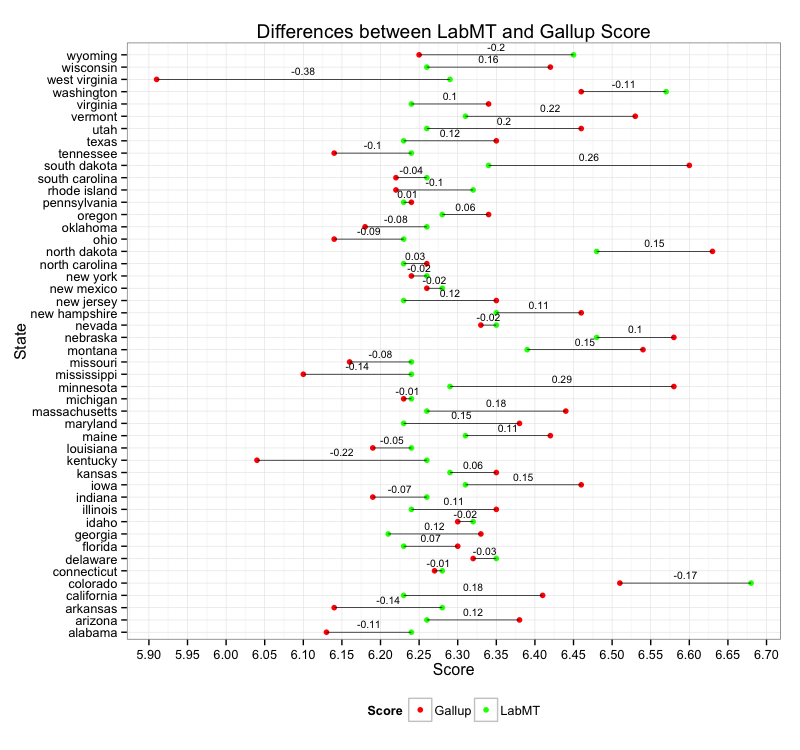
\includegraphics[width=\textwidth]{images/differences}
\caption{Difference in the score using our LabMT approach, and Gallup-Healthway Well-Being Index, rescaled to the range used in \cite{Dodds2009,Dodds2011} method, i.e. 1 to 9. I can see - just like it happen with the ranking - that when the difference is small, it is very small, and when the difference is large, it's significantly large.}
\label{fig:differences}
\end{figure}

\newgeometry{margin=1.1cm} % modify this if you need even more space
\begin{landscape}

% latex table generated in R 3.1.0 by xtable 1.7-3 package
% Sun Jun  1 00:04:06 2014
\begin{table}
\centering
\begin{tabular}{rlrrrrrrrrrrr}
  \hline
 State & Tweets & LabMT Ranking & Gallup Ranking & Gallup Score & Mode & Mode diff. & Median & Median diff. & Mean & Mean diff & Mode SD \\
  \hline
    colorado & 1854 &   1 &   1 & 6.58 & 6.68 & -0.10 & 6.24 & 0.34 & 6.00 & 0.58 & 1.15 \\
    washington & 2855 &   2 &  14 & 6.42 & 6.57 & -0.15 & 6.24 & 0.18 & 6.01 & 0.41 & 1.16 \\
    nebraska & 1059 &   3 &   6 & 6.48 & 6.48 & 0.00 & 6.22 & 0.26 & 5.97 & 0.51 & 1.14 \\
    north dakota & 445 &   4 &  18 & 6.39 & 6.48 & -0.09 & 6.16 & 0.23 & 5.89 & 0.50 & 1.08 \\
    wyoming & 187 &   5 &  12 & 6.43 & 6.45 & -0.02 & 6.19 & 0.24 & 5.88 & 0.55 & 1.24 \\
    montana & 141 &   6 &   5 & 6.48 & 6.39 & 0.09 & 6.20 & 0.28 & 5.85 & 0.63 & 1.29 \\
    delaware & 1607 &   7 &  25 & 6.33 & 6.35 & -0.02 & 6.24 & 0.09 & 5.95 & 0.38 & 1.15 \\
    nevada & 2999 &   8 &  37 & 6.22 & 6.35 & -0.13 & 6.32 & -0.10 & 6.10 & 0.12 & 1.08 \\
    new hampshire & 500 &   9 &   7 & 6.47 & 6.35 & 0.12 & 6.34 & 0.13 & 6.07 & 0.40 & 1.18 \\
    south dakota & 389 &  10 &  11 & 6.44 & 6.34 & 0.10 & 6.24 & 0.20 & 5.94 & 0.50 & 1.22 \\
    idaho & 262 &  11 &  22 & 6.37 & 6.32 & 0.05 & 6.33 & 0.04 & 6.16 & 0.21 & 1.16 \\
    rhode island & 897 &  12 &  36 & 6.24 & 6.32 & -0.08 & 6.18 & 0.06 & 5.87 & 0.37 & 1.21 \\
    iowa & 1992 &  13 &   8 & 6.45 & 6.31 & 0.14 & 6.28 & 0.17 & 6.04 & 0.41 & 1.19 \\
    maine & 416 &  14 &  19 & 6.38 & 6.31 & 0.07 & 6.24 & 0.14 & 5.95 & 0.43 & 1.14 \\
    vermont & 112 &  15 &   4 & 6.49 & 6.31 & 0.18 & 6.17 & 0.32 & 6.01 & 0.48 & 1.15 \\
    kansas & 1773 &  16 &  16 & 6.41 & 6.29 & 0.12 & 6.24 & 0.17 & 6.00 & 0.41 & 1.14 \\
    minnesota & 3458 &  17 &   2 & 6.51 & 6.29 & 0.22 & 6.27 & 0.24 & 6.03 & 0.48 & 1.15 \\
    west virginia & 1411 &  18 &  48 & 5.90 & 6.29 & -0.39 & 6.24 & -0.34 & 5.99 & -0.09 & 1.16 \\
    arkansas & 2275 &  19 &  44 & 6.13 & 6.28 & -0.15 & 6.24 & -0.11 & 5.98 & 0.15 & 1.11 \\
    connecticut & 3270 &  20 &  15 & 6.41 & 6.28 & 0.13 & 6.24 & 0.17 & 5.95 & 0.46 & 1.17 \\
    new mexico & 1099 &  21 &  24 & 6.34 & 6.28 & 0.06 & 6.17 & 0.17 & 5.92 & 0.42 & 1.15 \\
    oregon & 1679 &  22 &  23 & 6.37 & 6.28 & 0.09 & 6.25 & 0.12 & 6.06 & 0.31 & 1.14 \\
    arizona & 4970 &  23 &  21 & 6.37 & 6.26 & 0.11 & 6.26 & 0.11 & 6.05 & 0.32 & 1.13 \\
    indiana & 6790 &  24 &  40 & 6.21 & 6.26 & -0.05 & 6.24 & -0.03 & 5.99 & 0.22 & 1.14 \\
    kentucky & 4695 &  25 &  47 & 6.02 & 6.26 & -0.24 & 6.20 & -0.18 & 5.92 & 0.10 & 1.15 \\
    massachusetts & 6311 &  26 &   9 & 6.45 & 6.26 & 0.19 & 6.24 & 0.21 & 5.94 & 0.51 & 1.17 \\
    new york & 14910 &  27 &  29 & 6.30 & 6.26 & 0.04 & 6.26 & 0.04 & 6.00 & 0.30 & 1.15 \\
    oklahoma & 2440 &  28 &  38 & 6.22 & 6.26 & -0.04 & 6.21 & 0.01 & 5.90 & 0.32 & 1.17 \\
    south carolina & 7182 &  29 &  39 & 6.22 & 6.26 & -0.04 & 6.20 & 0.02 & 5.89 & 0.33 & 1.19 \\
    utah & 1482 &  30 &   3 & 6.50 & 6.26 & 0.24 & 6.22 & 0.28 & 5.97 & 0.53 & 1.11 \\
    wisconsin & 4288 &  31 &  20 & 6.38 & 6.26 & 0.12 & 5.89 & 0.49 & 5.82 & 0.56 & 1.08 \\
    alabama & 5431 &  32 &  43 & 6.14 & 6.24 & -0.10 & 6.24 & -0.10 & 5.98 & 0.16 & 1.14 \\
    illinois & 11490 &  33 &  26 & 6.33 & 6.24 & 0.09 & 6.23 & 0.10 & 5.93 & 0.40 & 1.17 \\
    louisiana & 6614 &  34 &  41 & 6.18 & 6.24 & -0.06 & 6.22 & -0.04 & 5.90 & 0.28 & 1.17 \\
    michigan & 11314 &  35 &  34 & 6.25 & 6.24 & 0.01 & 6.24 & 0.01 & 5.91 & 0.34 & 1.19 \\
    mississippi & 5992 &  36 &  46 & 6.09 & 6.24 & -0.15 & 6.18 & -0.09 & 5.85 & 0.24 & 1.22 \\
    missouri & 4758 &  37 &  35 & 6.24 & 6.24 & 0.00 & 6.21 & 0.03 & 5.91 & 0.33 & 1.17 \\
    tennessee & 6145 &  38 &  45 & 6.12 & 6.24 & -0.12 & 6.24 & -0.12 & 5.96 & 0.16 & 1.18 \\
    virginia & 11025 &  39 &  13 & 6.42 & 6.24 & 0.18 & 6.24 & 0.18 & 5.96 & 0.46 & 1.16 \\
    california & 27545 &  40 &  17 & 6.39 & 6.23 & 0.16 & 6.25 & 0.14 & 6.02 & 0.37 & 1.14 \\
    florida & 20522 &  41 &  32 & 6.26 & 6.23 & 0.03 & 6.24 & 0.02 & 5.95 & 0.31 & 1.16 \\
    maryland & 12143 &  42 &  10 & 6.44 & 6.23 & 0.21 & 6.22 & 0.22 & 5.89 & 0.55 & 1.20 \\
    new jersey & 12450 &  43 &  31 & 6.29 & 6.23 & 0.06 & 6.24 & 0.05 & 5.96 & 0.33 & 1.16 \\
    north carolina & 13979 &  44 &  33 & 6.26 & 6.23 & 0.03 & 6.22 & 0.04 & 5.93 & 0.33 & 1.17 \\
    ohio & 15368 &  45 &  42 & 6.17 & 6.23 & -0.06 & 6.22 & -0.05 & 5.92 & 0.25 & 1.19 \\
    pennsylvania & 15205 &  46 &  28 & 6.32 & 6.23 & 0.09 & 6.24 & 0.08 & 5.94 & 0.38 & 1.17 \\
    texas & 33855 &  47 &  27 & 6.33 & 6.23 & 0.10 & 6.22 & 0.11 & 5.88 & 0.45 & 1.20 \\
    georgia & 24199 &  48 &  30 & 6.29 & 6.21 & 0.08 & 6.21 & 0.08 & 5.89 & 0.40 & 1.16 \\
   \hline
\end{tabular}
\caption{Table with all the ranking and scores data for each state. The `diff' are always relatively to Gallup-Healthway score.}
\end{table}

\end{landscape}
\restoregeometry


\end{document}
